\section{Derivation of the Jacobian}

\begin{frame}[standout, plain, noframenumbering]
    Derivation of the Jacobian

    % \medskip

    % \footnotesize
    % Sam Greydanus \quad Misko Dzamba \quad Jason Yosinski
\end{frame}

\begingroup
\small


\begin{frame}
    \frametitle{Derivation of the Jacobian}

    \begin{itemize}
        \item Consider an $n$-link manipulator with joint variables $q_1, \ldots, q_n$. Let
        \[ T_n^0 = \bmat{R_n^0(q) & o_n^0(q) \\ 0 & 1} \] denote the
            transformation from the end effector frame $\Sigma_n$ to the base
            frame $\Sigma_0$.
        \item The objective of this section is to relate the linear and angular
        velocity of the end effector $\Sigma_n$ to the vector of joint
        velocities $\dot{q}(t)$. 
        \item Let \[ S\left( \omega_n^0 \right) = \dot{R}_n^0 \left( R_n^0 \right)^\top, \]
        denote the angular velocity vector $\omega_n^0$ of the end effector, and let
        \[ v_n^0 = \dot{o}_n^0, \] denote the linear velocity of the end effector.
    \end{itemize}
\end{frame}


\begin{frame}
    \frametitle{Derivation of the Jacobian}

    \begin{itemize}
        \item We seek expressions of the form
        \begin{align}
            v_n^0 &= J_v\dot{q} \label{eq:def_jac_v}, \\
            \omega_n^0 &= J_\omega\dot{q} \label{eq:def_jac_omega},
        \end{align}
        where $J_v, J_\omega \in \mathbb{R}^{3 \times n}$. Together, they can be
        written as 
        \[ \xi = J\dot{q}, \] in which $\xi$ and $J$ (\textbf{manipulator
        Jacobian} or \textbf{Jacobian}) are given by 
        \[ \xi = \bmat{v_n^0 \\ \omega_n^0} \quad \text{and} \quad J = \bmat{J_v \\ J_\omega}_{6 \times n}. \]
        \item This velocity vector $\xi$ is \textsc{not} the derivative of a
        position variable, since the angular velocity vector is not the
        derivative of any particular time-varying quantity.
    \end{itemize}
\end{frame}


\begin{frame}
    \frametitle{Angular Velocity}

    \begin{itemize}
        \item We can determine $\omega_{0,n}^0$ by expressing the angular velocity 
        contributed by each joint in $\Sigma_0$ and then summing these.
        \item If the joint $i$ is revolute, then the $i^{\textrm{th}}$ variable 
        $q_i$ equals $\theta_i$ and the axis of rotation is $z_{i-1}$.
        \item Recall $\omega_{i-1,i}^{i-1}$ represents the angular velocity of
        link $i$ that is imparted by the rotation of joint $i$, expressed
        relative to frame $\Sigma_{i-1}$. We have with $k = (0, 0, 1)$,
        \[ \omega_{i-1,i}^{i-1} = \dot{q}_i z_{i-1}^{i-1} = \dot{q}_ik. \]
        \item If the joint $i$ is prismatic, then the motion of $\Sigma_i$
        w.r.t. $\Sigma_1$ is a translation and \[ \omega_{i-1,i}^{i-1} = 0. \]
    \end{itemize}
\end{frame}

\begin{frame}
    \frametitle{Angular Velocity}

    \begin{itemize}
        \item Therefore, the overall angular velocity of the end effector
        $\omega_{0,n}^0$ is determined by 
        \begin{align*}
            \omega_{0,n}^0 &= \omega_{0,1}^0 + R_1^0\omega_{1,2}^1 + R_2^0\omega_{2,3}^2 + \cdots + R_n^0\omega_{n-1,n}^{n-1} \\ 
            &= \rho_1 \dot{q}_1k + \rho_2 \dot{q}_2R_1^0k + \cdots + \rho_n\dot{q}_nR_{n-1}^0k = \sum_{i=1}^n \rho_i \dot{q}_i z_{i-1}^0,
        \end{align*}
        in which $\rho_i$ is equal to $1$ if joint $i$ is revolute and $0$ if
        joint $i$ is prismatic, since $z_{i-1}^0 = R_{i-1}^0k$.
        \item Hence, we have found $J_\omega$ as 
        \begin{equation}
            J_\omega = \bmat{\rho_1 z_0 & \cdots & \rho_n z_{n-1}}.
            \label{eq:jac_omega}
        \end{equation}
        where all $z$-axes are expressed in the world frame $\Sigma_0$.
    \end{itemize}
\end{frame}


\begin{frame}
    \frametitle{Linear Velocity}

    % \begin{columns}
        % \begin{column}{0.6\textwidth}
            \begin{itemize}
                \item By the chain rule for differentiation \[
                \dot{o}_n^0 = \sum_{i=1}^n \pd{o_n^0}{q_i}\dot{q}_i.
                \]
                \item Thus, the $i^{\textrm{th}}$ column, $J_{v_i}$, of $J_v$ is 
                given by \[ J_{v_i} = \pd{o_n^0}{q_i}. \]
                \item Note that the $i^{\textrm{th}}$ column, $J_{v_i}$, of the
                Jacobian may be generated by holding all joints but the
                $i^{\textrm{th}}$ fixed and actuating the $i^{\textrm{th}}$ at 
                unit velocity.
            \end{itemize}
        % \end{column}
        % \begin{column}{0.4\textwidth}
        %     \begin{figure}[bth]
        %         \centering
        %         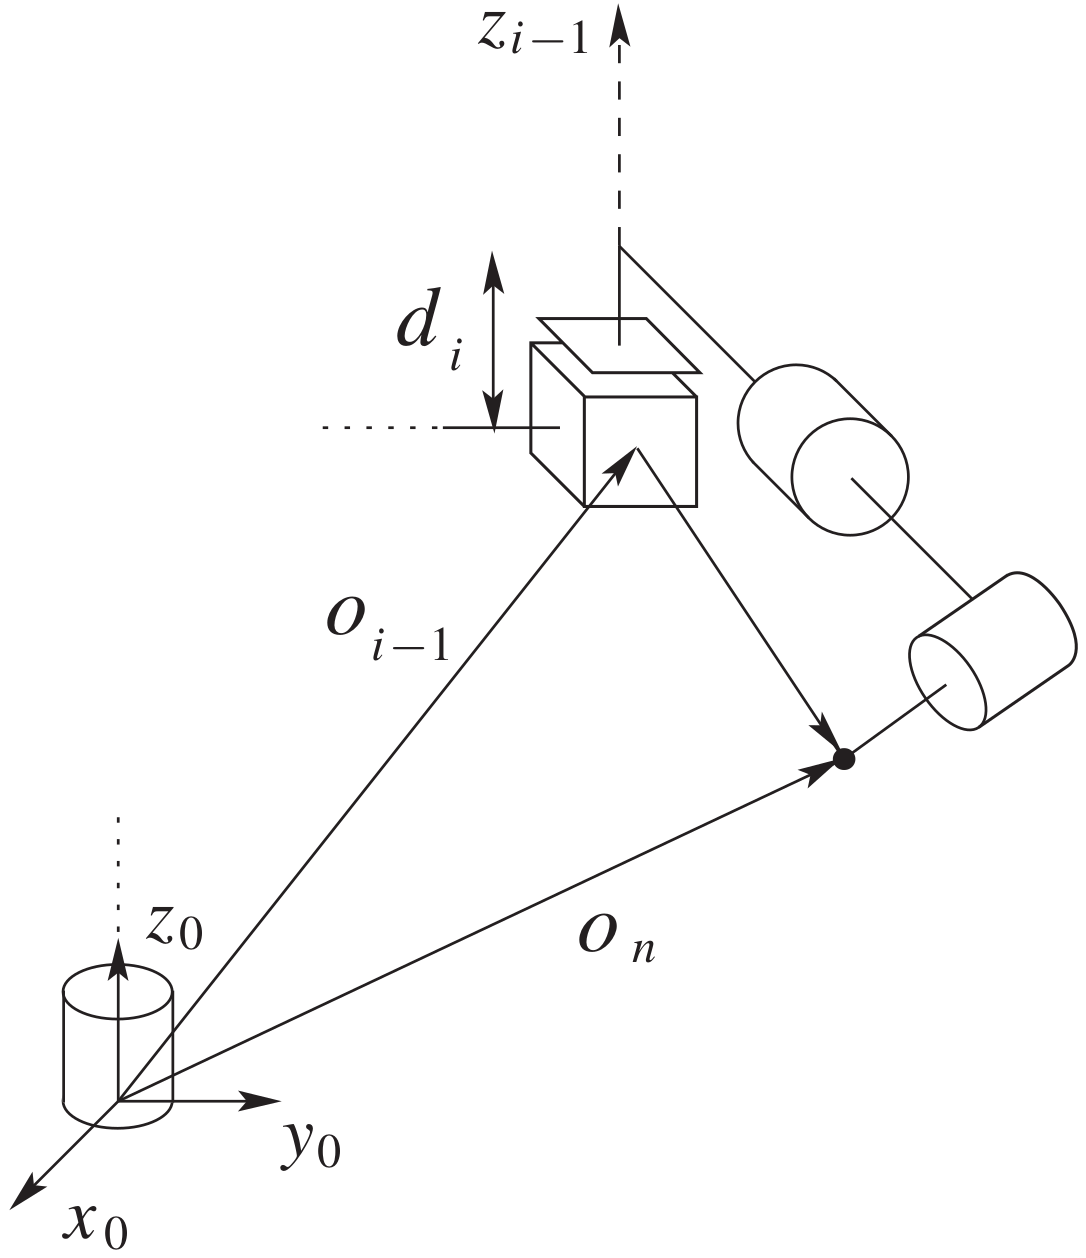
\includegraphics[width=0.95\textwidth]{figures/motion_due_to_prismatic.png} 
        %         % \caption{\footnotesize }
        %     \end{figure}
            % \vspace{-3mm}
        %     \centering
        %     \footnotesize{Motion of the end effector due to prismatic joint $i$.}
        % \end{column}
    % \end{columns}
\end{frame}


\begin{frame}
    \frametitle{Linear Velocity: Prismatic Joints}

    \begin{columns}
        \begin{column}{0.6\textwidth}
            \begin{itemize}
                \item Since joint $i$ is prismatic, it imparts a pure translation 
                to the end effector.
                \item The direction of this translation is $\parallel$ to
                $z_{i-1}$ and the magnitude is $\dot{d}_i$.
                \item Thus, expressed in $\Sigma_0$, we have
                \[ \dot{o}_n^0 = \dot{d}_iR_{i-1}^0\bmat{0 \\ 0 \\ 1} = \dot{d}_iz_{i-1}^0, \]
                in which $d_i$ is the joint variable for prismatic joint $i$.
                \item After dropping the superscripts, we have \[ J_{v_i} =
                z_{i-1}. \]
            \end{itemize}
        \end{column}
        \begin{column}{0.4\textwidth}
            \begin{figure}[bth]
                \centering
                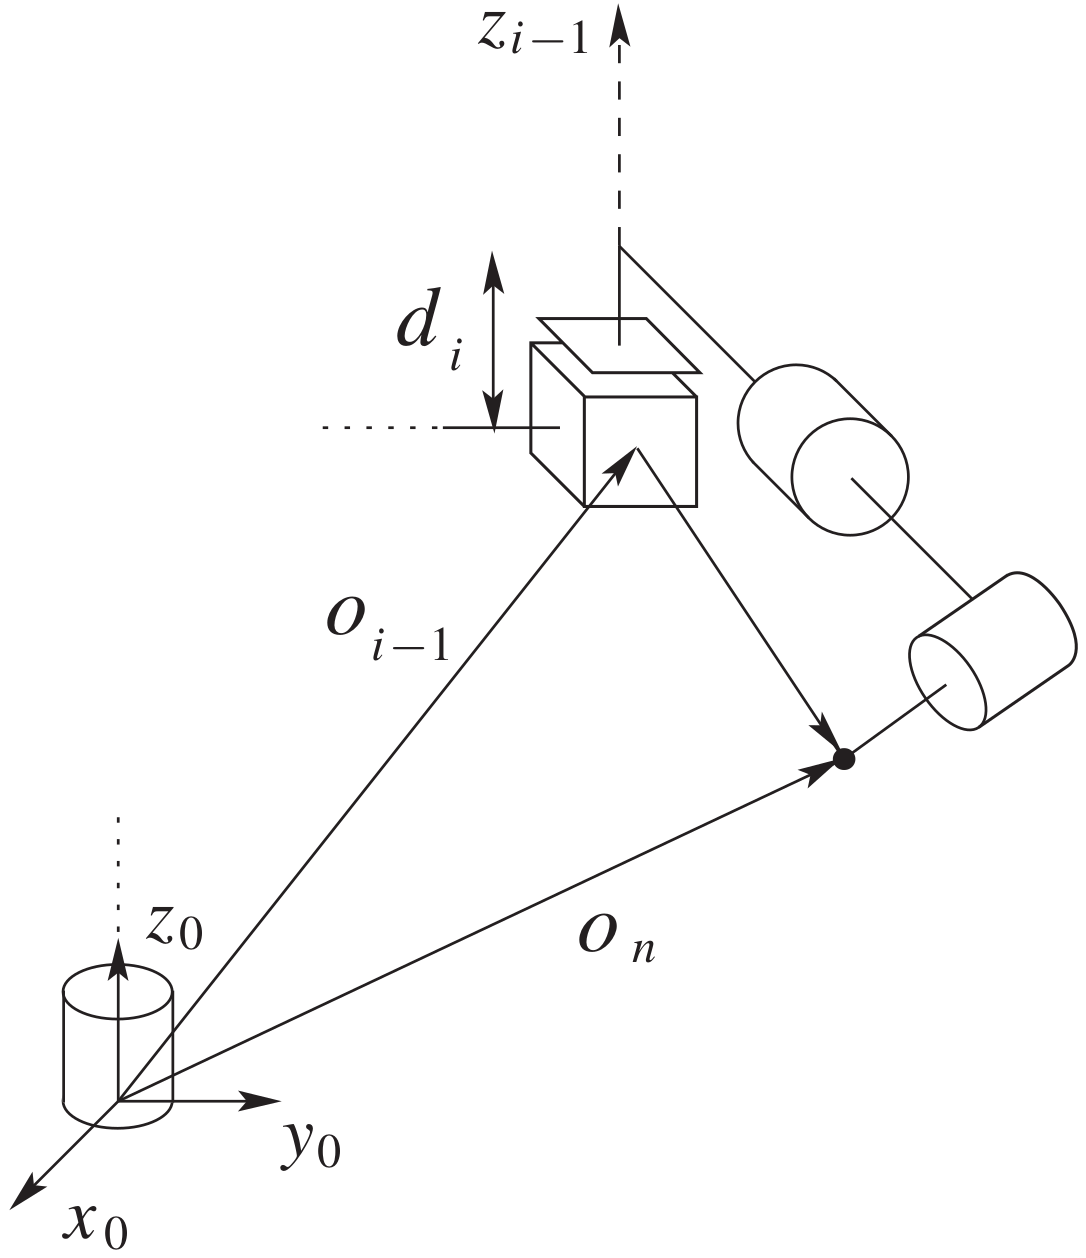
\includegraphics[width=0.95\textwidth]{figures/motion_due_to_prismatic.png} 
                % \caption{\footnotesize }
            \end{figure}
            \vspace{-3mm}
            \centering
            \footnotesize{Motion of the end effector due to prismatic joint $i$.}
        \end{column}
    \end{columns}
\end{frame}



\begin{frame}
    \frametitle{Linear Velocity: Revolute Joints}

    \begin{columns}
        \begin{column}{0.6\textwidth}
            \begin{itemize}
                \item Since joint $i$ is revolute, we have $q_i = \theta_i$.
                \item We see that the linear velocity of the end effector is
                simply of the form $\omega \times r$, where \[ \omega =
                \dot{\theta}_i z_{i-1}, \] and \[ r = o_n - o_{i-1}. \]
                \item Putting these together and expressing the coordinates
                relative to $\Sigma_0$, for a revolute joint we obtain
                \[ J_{v_i} = z_{i-1} \times (o_n - o_{i-1}). \]
            \end{itemize}
        \end{column}
        \begin{column}{0.4\textwidth}
            \begin{figure}[bth]
                \centering
                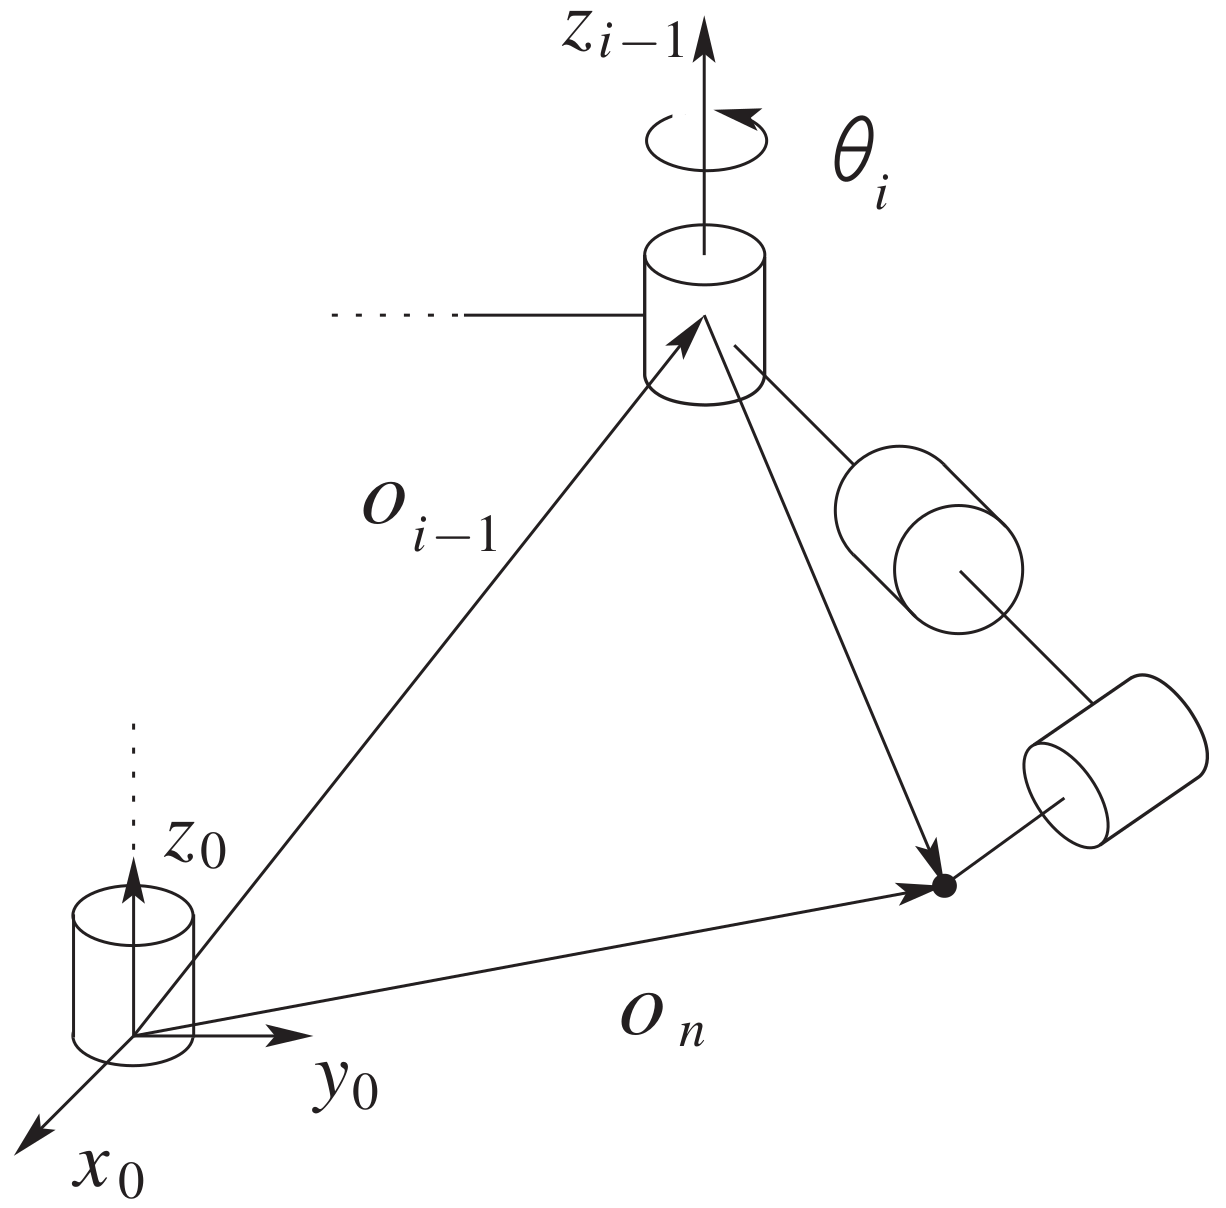
\includegraphics[width=0.95\textwidth]{figures/motion_due_to_revolute.png} 
                % \caption{\footnotesize }
            \end{figure}
            \vspace{-3mm}
            \centering
            \footnotesize{Motion of the end effector due to revolute joint $i$.}
        \end{column}
    \end{columns}
\end{frame}



\begin{frame}
    \frametitle{Combining Linear and Angular Velocity Jacobians}

    \begin{itemize}
        \item The upper half, $J_v$, of the Jacobian $J$ is given as \[ J_v =
        \bmat{J_{v_1} \cdots J_{v_n}}, \] in which the $i^{\textrm{th}}$ column
        $J_{v_i}$ is \[ J_{v_i} = 
        \begin{cases}
            z_{i-1} \times (o_n - o_{i-1}) & \mbox{for revolute joint $i$} \\
            z_{i-1} & \mbox{for prismatic joint $i$}
        \end{cases}    
        \]
        \item The lower half, $J_\omega$, of the Jacobian $J$ is given as
        \[J_\omega = \bmat{J_{\omega_1} \cdots J_{\omega_n}} \] in which the
        $i^{\textrm{th}}$ column $J_{\omega_i}$ is \[ J_{\omega_i} = 
        \begin{cases}
            z_{i-1} & \mbox{for revolute joint $i$} \\
            0 & \mbox{for prismatic joint $i$}
        \end{cases}
        \]
    \end{itemize}
\end{frame}


\begin{frame}
    \frametitle{Combining Linear and Angular Velocity Jacobians}

    \begin{itemize}
        \item The only quantities needed to compute the Jacobian are the unit 
        vectors $z_i$ and the coordinates of the origin $o_1, \ldots, o_n$.
        \item The coordinates for $z_i$ w.r.t. $\Sigma_0$ are given by the first 
        three elements in the third column of $T_i^0$.
        \item $o_i$ is given by the first three elements of the fourth column of 
        $T_i^0$.
        \item This procedure works not only for computing the velocity of the
        end effector but also for computing the velocity of any point on the
        manipulator.
    \end{itemize}
\end{frame}


\begin{frame}
    \frametitle{Example 4.5: Two-Link Planar Manipulator}
    \begin{columns}
        \begin{column}{0.6\textwidth}
            \only<1>{
            \begin{itemize}
                \item Since both joints are revolute, the Jacobian matrix is of the form
                \[
                J(q) = \bmat{
                    z_0 \times (o_2-o_0) & z_1 \times (o_2-o_1) \\ 
                    z_0 & z_1
                }    
                \]
                \item The various quantities are
                \[ z_0 = z_1 = \bmat{0 \\ 0 \\ 1}. \]
                \[
                o_0 = 0, \;\; o_1 = \bmat{a_1c_1 \\ a_1s_1 \\ 0}, \;\; o_2 = \bmat{
                    a_1c_1 + a_2c_{12} \\ a_1s_1 + a_2s_{12} \\ 0
                }
                \]
            \end{itemize}
            }
            \only<2>{
            \begin{itemize}
                \item The first two rows give the linear velocity of the origin 
                $o_2$ relative to the base.
                \item The third row is the linear velocity in the direction of
                $z_0$.
                \item The last three rows represent the angular velocity of the
                final frame, $\Sigma_2$, which is a basic rotation about the 
                vertical axis at the rate $\dot{\theta}_1 + \dot{\theta}_2$.
            \end{itemize}
            }
        \end{column}
        \begin{column}{0.4\textwidth}
            \begin{figure}[bth]
                \centering
                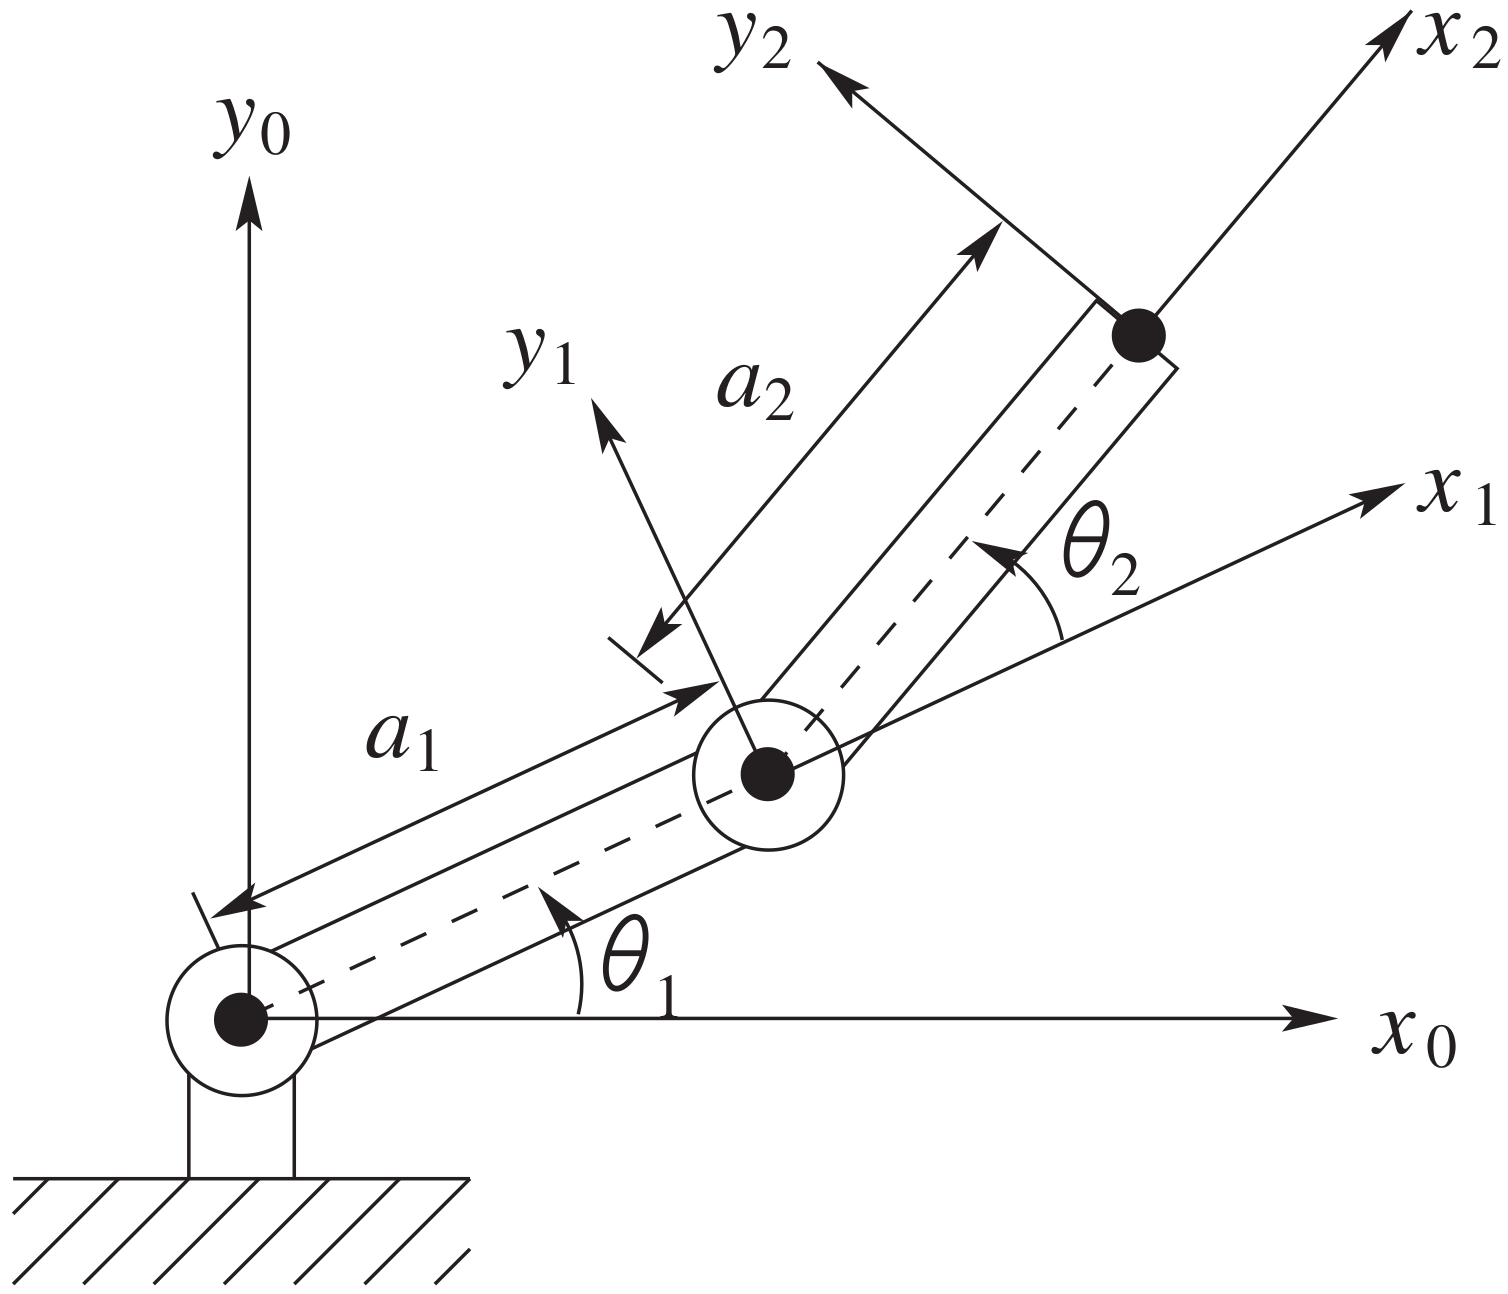
\includegraphics[width=0.85\textwidth]{figures/two_link_planar_manipulator.png} 
                % \caption{\footnotesize }
            \end{figure}
            \vspace{-2mm}
            \centering
            \footnotesize{Two-link planar manipulator.}
            \only<2>{
            \[
            J = \bmat{
                -a_1s_1 - a_2s_{12} & -a_2s_{12} \\
                a_1c_1 + a_2c_{12} & a_2c_{12} \\
                0 & 0 \\
                0 & 0 \\
                0 & 0 \\
                1 & 1
            }    
            \]
            }
        \end{column}
    \end{columns}
\end{frame}

\begin{frame}
    \frametitle{Example 4.6: Jacobian for an Arbitrary Point on a Link}
   
    \begin{columns}
        \begin{column}{0.6\textwidth}
            \only<1>{
            \begin{itemize}
                \item Suppose we wish to compute the linear velocity $v$ and the
                angular velocity $\omega$ of the center of link $2$ as shown.
                \[
                    \footnotesize{
                J(q) = \bmat{
                    z_0 \times (o_c-o_0) & z_1 \times (o_c-o_1) & 0 \\ 
                    z_0 & z_1 & 0
                }    
                    }
                \]
                which is merely the Jacobian with $o_c$ in place of $o_n$.
                \item The third column of the Jacobian is zero, since the
                velocity of the second link is unaffected by the motion of the 
                third link.
            \end{itemize}
            }
            % \only<2>{
            % \begin{itemize}
            %     \item The first two rows give the linear velocity of the origin 
            %     $o_2$ relative to the base.
            %     \item The third row is the linear velocity in the direction of
            %     $z_0$.
            %     \item The last three rows represent the angular velocity of the
            %     final frame, $\Sigma_2$, which is a basic rotation about the 
            %     vertical axis at the rate $\dot{\theta}_1 + \dot{\theta}_2$.
            % \end{itemize}
            % }
        \end{column}
        \begin{column}{0.4\textwidth}
            \begin{figure}[bth]
                \centering
                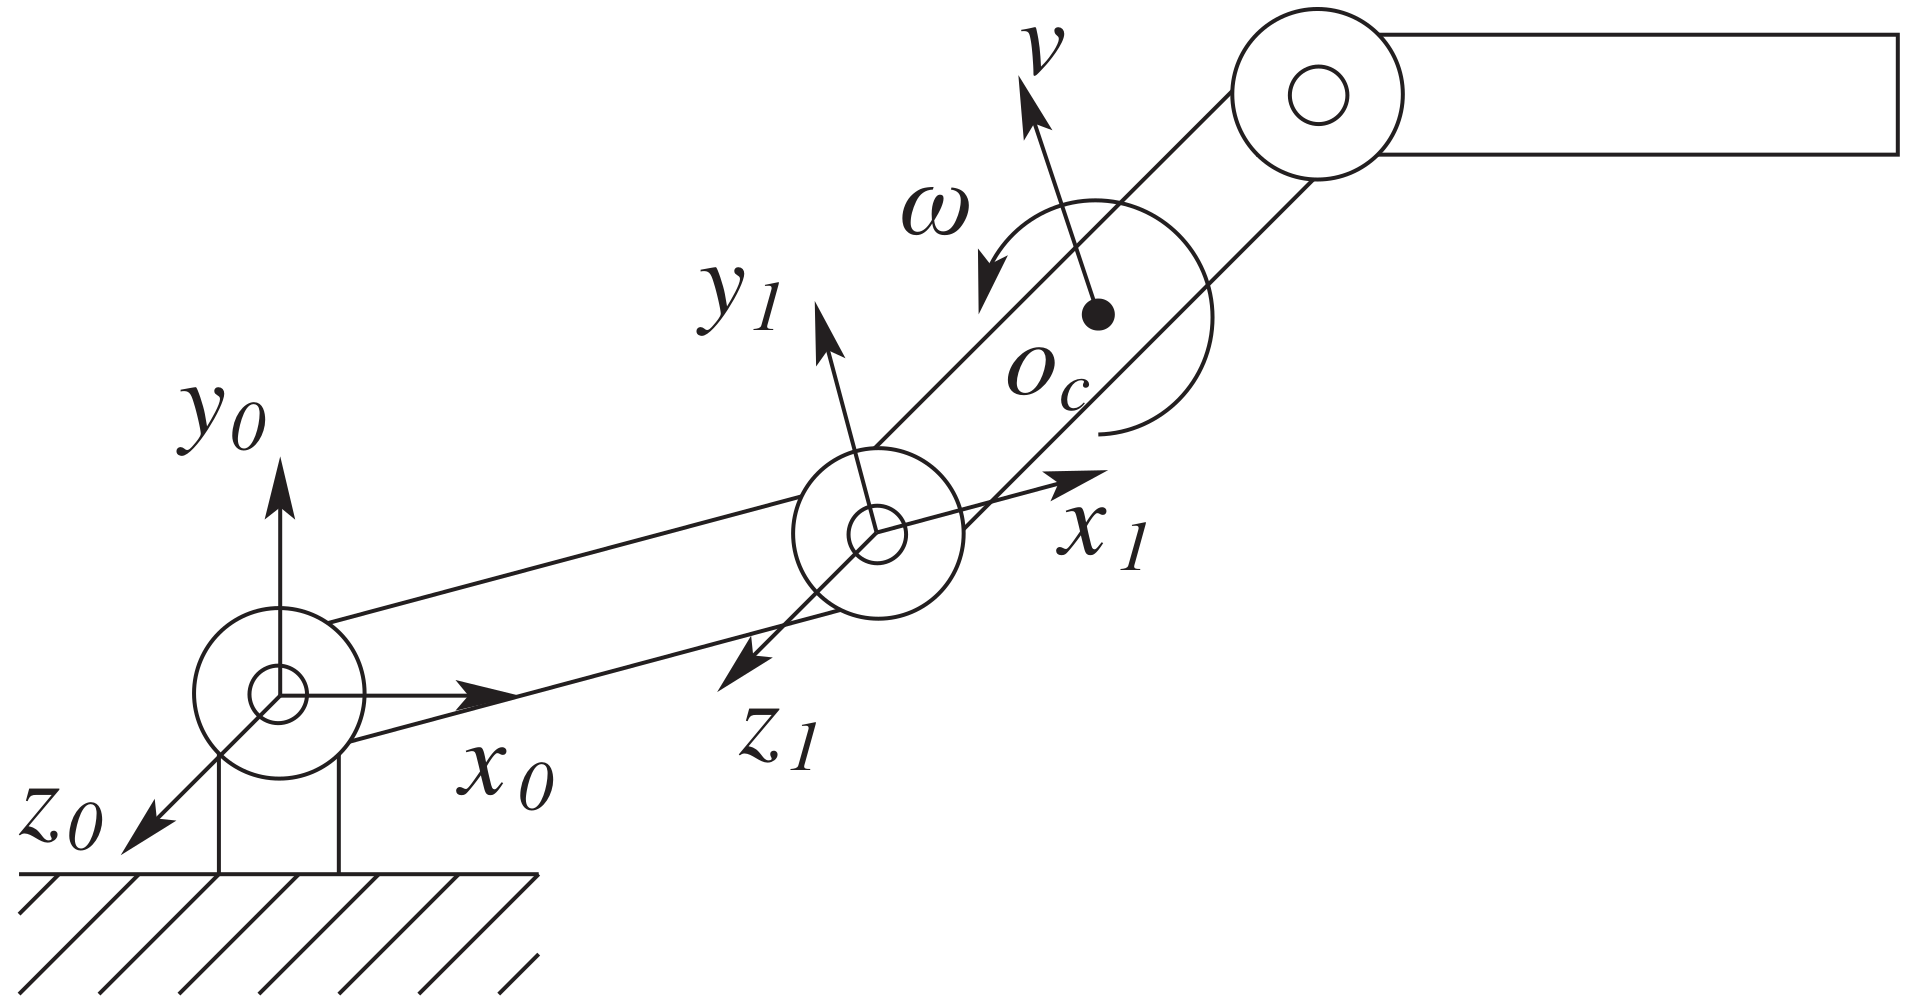
\includegraphics[width=0.85\textwidth]{figures/vel_of_planar_robot.png} 
                % \caption{\footnotesize }
            \end{figure}
            \vspace{-2mm}
            \centering
            \footnotesize{Finding the velocity of link $2$ of a $3$-link planar robot.}

            \begin{itemize}
                \item In this case the vector $o_c$ must be computed as it is 
                not given directy by the $T$ matrices.
            \end{itemize}
        \end{column}
    \end{columns}
\end{frame}

\begin{frame}
    \frametitle{Example 4.7: Stanford Manipulator}
   
    \begin{itemize}
        \item Joint $3$ is prismatic and $o_3 = o_4 = o_5$ as a consequence of 
        the spherical wrist and frame assignment.
        \item Denoting this common origin by $o$, we see that the columns of the 
        Jacobian have the form

        \begin{align*}
            J_i &= \bmat{z_{i-1} \times (o_6 - o_{i-1}) \\ z_{i-1}}, \; \; i = 1,2, \\
            J_3 &= \bmat{z_2 \\ 0} \\
            J_i &= \bmat{z_{i-1} \times (o_6 - o) \\ z_{i-1}}, \; \; i = 4,5,6.
        \end{align*}
    \end{itemize}
\end{frame}

\begin{frame}
    \frametitle{Example 4.8: SCARA Manipulator}
   
    \begin{itemize}
        \item This Jacobian is a $6 \times 4$ matrix since SCARA has only four 
        degrees of freedom.
        \item We need only compute the matrices $T_j^0 = A_1 \cdots A_j$.
        \item Since joints $1$, $2$, and $4$ are revolute and joint $3$ is
        prismatic, and since $o_4 - o_3 \parallel z_3$ (and thus $z_3 \times
        (o_4 - o_3) = 0$), the Jacobian is of the form
        \begin{align*}
        J &= \bmat{
            z_0 \times (o_4 - o_0) & z_1 \times (o_4 - o_1) & z_2 & 0 \\ 
            z_0 & z_1 & 0 & z_3
        } \\
        &= \bmat{
            -a_1s_1 - a_2s_{12} & -a_2s_{12} & 0 & 0 \\
            a_1c_1 + a_2c_{12} & a_2c_{12} & 0 & 0 \\
            0 & 0 & -1 & 0 \\
            0 & 0 & 0 & 0 \\
            0 & 0 & 0 & 0 \\
            1 & 1 & 0 & -1
        }.
        \end{align*}
    \end{itemize}

\end{frame}

\endgroup